\cotefile{147}
\scanpage{134}
\mspage{66}

terms, one must introduce, \deleted{\unsure{some cases}}
for a morphism
\diagram{(218)\qquad
\begin{tikzcd}[ampersand replacement=\&]
\Delta_r \arrow[r,no head,"\alpha"] \& \Delta_{r'}
\end{tikzcd},}
a \uline{corresponding morphism} of groupoids
\diagram{(219)\qquad
\fbox{\begin{tikzcd}[ampersand replacement=\&]
\widetilde{\Pi}_{\Delta_{r'}} \arrow[r,"\widetilde{\alpha}^{*}"]
\& \Pi_{\Delta_r}
\end{tikzcd}}}
which will be called the \uline{generization homomorphism}
associated with $\alpha$.
\margin{\figure{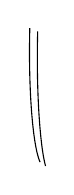
\begin{tikzpicture}
\draw (0,1.7) .. controls (-.02,.9) and (.04,.2) .. (.13,0);
\draw (.10,1.66) .. controls (.08,.9) and (.13,.2) .. (.20,-.05);
\end{tikzpicture}}}
Since $\alpha$ factors
canonically as a surjective homomorphism
followed by an injective homomorphism of simplices,
we are reduced to examining separately
the two cases. But if $\alpha$ is surjective
(``degeneracy homomorphism''), \deleted{the homomorphism}
\inserted{we have $\alpha(0)=0$}
so we are in the case already considered --
\deleted{\unsure{corresponding}}\inserted{moreover} in this case
\diagram{\begin{tikzcd}[ampersand replacement=\&]
D^*_{\Delta_{r'}} \arrow[r] \& D^*_{\Delta_r}
\end{tikzcd}}
\unsure{is|has|to} decomposed into morphisms \unsure{:|;}
\diagram{(220)\qquad
\begin{tikzcd}[ampersand replacement=\&]
D^*_{d'_0,\unsure{\ldotp-\!-|-\!-},d'_{r'}}
\arrow[r] \&
D^*_{\unsure{d_0^{\deleted{\prime}}|d_0^*},-\!-,\unsure{d_r^{\deleted{\prime}}|d_r^*}}
\end{tikzcd},}
$(d_0,-\!-,d_r)$ is \unsure{obtained|obtained} from $(d'_0,-,d'_r)$
by \unsure{rewriting} this sequence, repeating some
of its elements -- and \deleted{the} then (220) is
an isomorphism -- so \uline{if $\alpha$ is a homomorphism}
\margin{We see that the consideration of the
$\widetilde{\Pi}_{d_0-d_r}$, $\Pi_{d_0,-d_r}$
for $d_0,-\!-,d_r$ \unsure{not}
\unsure{\uline{strictly}|\uuline{strictly}}
decreasing and that of $\alpha^*$, for $\alpha$
\unsure{not} \uline{strictly} increasing,
is eyewash, simply!}
\margin{133}
